
\documentclass{article}    % This document style supports \chapter
\usepackage{graphicx}

\textwidth 6.0in           % Real length of the printed page
\textheight=8.6in          % Real height of the printed page 
\hoffset=-0.9in            % These offsets is defined with respect to the 
\voffset=-0.7in            % ORIGINAL latex output. This is why they are 
\parindent=0in
                           % negative

\parskip=6pt               % separation between paragraphs

\lineskip=14pt             % separation between lines. The default is
\baselineskip=14pt         % the pointsize +2 (in this case 12pt).
                           % The extra 2 pts give more room for subindices
                           % and make the output look nicer. Double space
                           % is 24pts.

\title{A Benchmark of Question-Answering Problems about Two-Dimensional
Abstract Diagrams}
\author{Ernest Davis}
\begin{document}
\maketitle
\section*{Summary}
I have written code to generate random diagrams tiles with polygonal shapes
and random questions about these within 24 different general templates,
with the correct answers.
I believe that the problems are mostly easy for people and I conjecture 
that the current (August 2024) generation of visual QA systems would not
succeed at human levels. I am looking for collaborators to take this
project further.

This document is structured as follows:
\begin{itemize}
\item[1.] Examples of ten diagrams with questions (section~\ref{secExamples}).
The first diagram has examples
of all 24 types of questions: the remaining nine diagrams have 5
questions each.

\item[2.] Discussion (section~\ref{secBenchmark} of the current 
state of the benchmark: the characteristics of
the diagrams (section~\ref{secDiagrams}), the questions 
(section~\ref{secQuestions}) and the state of the code (section~\ref{secCode}).

\item[3.] Discussion (section~\ref{secFuture}) of various options for
taking this forward.
\end{itemize}

\section{Examples}
\label{secExamples}

Let me start by showing some examples, with associated questions and answers.

\subsection{Example 1}
\begin{center}
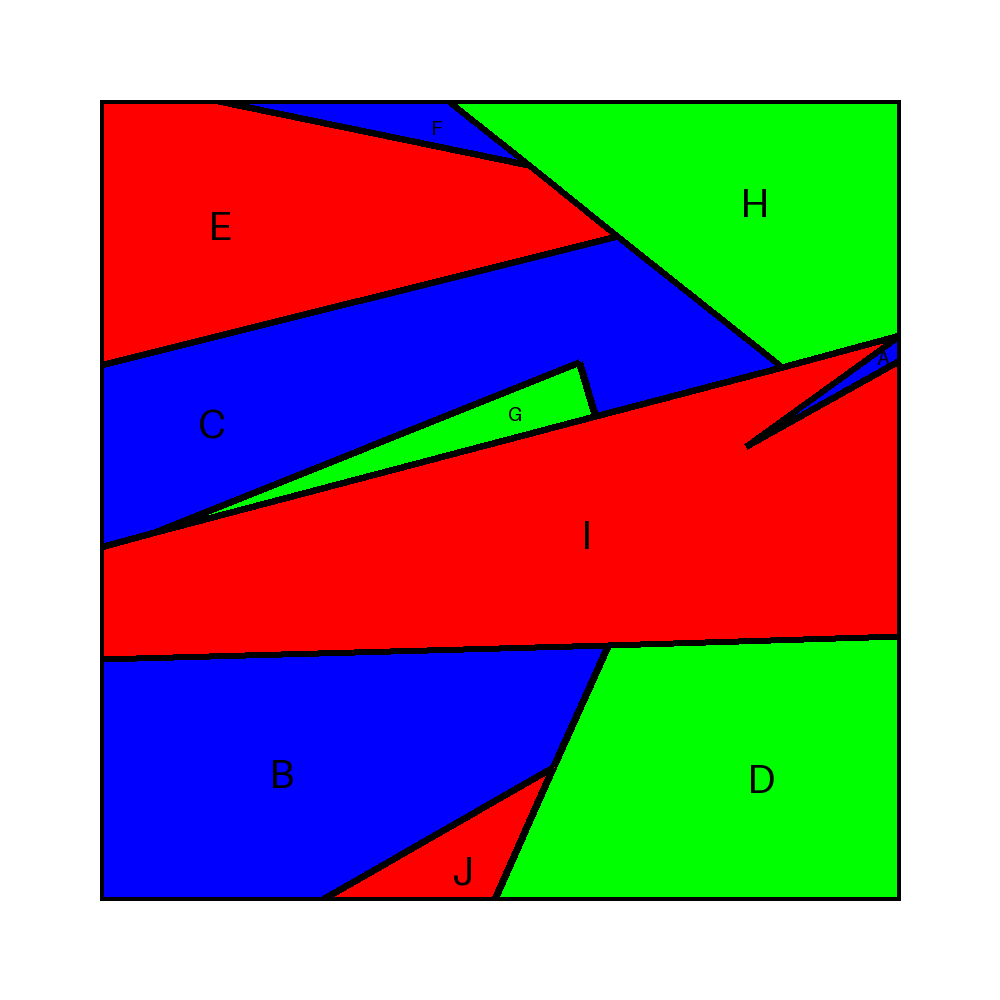
\includegraphics[height=4in]{Maps/RandomSetup9.png}
\end{center}

{\small  The diagram was created with the function 
call {\tt TestQuestions.randomSetup(9)}.
	The argument to {\tt randomSetup} is a seed for the random 
	number generator.}

{\small All example questions were generated with the function call \\
{\tt RandomQuestion.displayRandomQuestion($<$question number$>$, 1)}.
The second argument is the random seed.}

{\bf Question 1:}
Which regions border region B along an edge? \\
{\bf Answer:}
{I, J, D}

{\bf Question 2:}
If you draw a straight line segment from a point in the interior of region E to  a point in the interior of B, which other regions might it go through? \\
{\bf Answer:}
{G, I, C}

{\bf Question 3:}
Which if any of the regions are not convex? \\
{\bf Answer:}
{I, C}

{\bf Question 4:}
Let p be the rightmost vertex of J. Suppose that someone starts at p and goes counterclockwise around B until they have returned to p. What regions do they pass on their right in sequence? For this question, include the outside of the frame. \\
{\bf Answer:}
[D, I, Outside, J]

{\bf Question 5:}
Which pairs of regions, if any, meet at a vertex but not along an edge? \\
{\bf Answer:}
{(H, A)}

{\bf Question 6:}
Which pairs of regions, if any, meet along two or more disconnected edges? Do not include the outside of the frame. \\
{\bf Answer:}
{(I, C)}

{\bf Question 7:}
Which regions, if any, meet the outside of the frame along two or more disconnected edges? \\
{\bf Answer:}
{I}

{\bf Question 8:}
Which regions have 4 sides? \\
{\bf Answer:}
{H, D}

{\bf Question 9:}
How many sides does region B have? \\
{\bf Answer:}
5

{\bf Question 10:}
Let p be the meeting point of regions E and C with the outside of the frame. Let u be the rightmost vertex of F. Let v be the meeting point of regions C and I with the outside of the frame. Let w be the meeting point of regions H, I, and A with the outside of the frame.  Sort u,v,w in increasing order of distance from p.
{\bf Answer:}
['v', 'u', 'w']

{\bf Question 11:}
Region H has 4 vertices:  the vertex at the top right of the overall diagram; (2) the leftmost vertex of H; (3) the meeting point of H, C, and I; (4) the meeting point of H, I, and A with the outside of the frame. Sort these in increasing order by the size of the interior angle at each corner. \\
{\bf Answer:}
[2, 1, 4, 3]

{\bf Question 12:}
Let m be the edge of J that meets region B. Suppose m is extended in both directions along straight line L. Which are the regions R in the diagram for which L passes through the interior of R? (Do not include a region R if L only aligns with the boundary of R, and does not go through R's interior) \\
{\bf Answer:}
['D', 'I']

{\bf Question 13:}
Let p be the leftmost vertex of A. Which regions meet at p? \\
{\bf Answer:}
['A', 'I']

{\bf Question 14:}
Let U be the union of regions D and J. How many sides does U have? \\
{\bf Answer:}
5

{\bf Question 15:}
Let U be the union of regions D and J. Which of the labelled regions A-J does U border on an edge? \\
{\bf Answer:}
{B, I}

{\bf Question 16:}
Let N be the union of regions E and C. Sort regions [N, A, H] in order of increasing area: \\
{\bf Answer:}
[A, H, N]

{\bf Question 17:}
Find all pairs of regions <X,Y> with X!=Y such that the union of X and Y is convex. (There may be no such pairs.) \\
{\bf Answer:}
{(A, I), (J, B), (F, E), (G, C)}

{\bf Question 18:}
Let p be the rightmost vertex of J. Let q be the leftmost vertex of F. If you travel in a straight line from p to q, what regions do you pass through in the interior, in sequence? (If you enter and exit a region more than once, list it multiple times.) \\
{\bf Answer:}
[B, I, G, C, E]

{\bf Question 19:}
Let p be the topmost vertex of J. Suppose that you travel in a vertical line downward from p until you reach the bottom of the frame. What regions do you pass through in the interior, in sequence? (If you enter and exit a region more than once, list it multiple times.) \\
{\bf Answer:}
[D]

{\bf Question 20:}
Let u be the bottommost vertex of F. Let v be the bottommost vertex of G. Let w be the vertex of A with the widest angle. Order u, v, and w in order bottom to top. \\
{\bf Answer:}
[v, w, u]

{\bf Question 21:}
Let u be the meeting point of regions E and C with the outside of the frame. Let v be the vertex of H with the widest angle. Let w be the top left vertex of E. Suppose that someone travels from u to v to w back to u.Is this cycle clockwise or counterclockwise? \\
{\bf Answer:}
counterclockwise

{\bf Question 22:}
Let p be the vertex of F with the widest angle. Let q be the vertex at the top right of the overall diagram. Let u be the topmost vertex of J. Let v be the meeting point of regions C and I with the outside of the frame. Does the line segment between p and q cross the line segment between u and v? \\
{\bf Answer:}
No



{\bf Question 23:}
List all pairs of regions $<$X.Y$>$ such that the bottom vertex of X is the same as the top vertex of Y. \\
{\bf Answer:}
None

{\bf Question 24:}
Which region is closer to E: B or G? (Consider the distance between two regions to be the distance between their closest points.) \\
{\bf Answer:}
G

\pagebreak

\subsection{Example 2}
\begin{center}
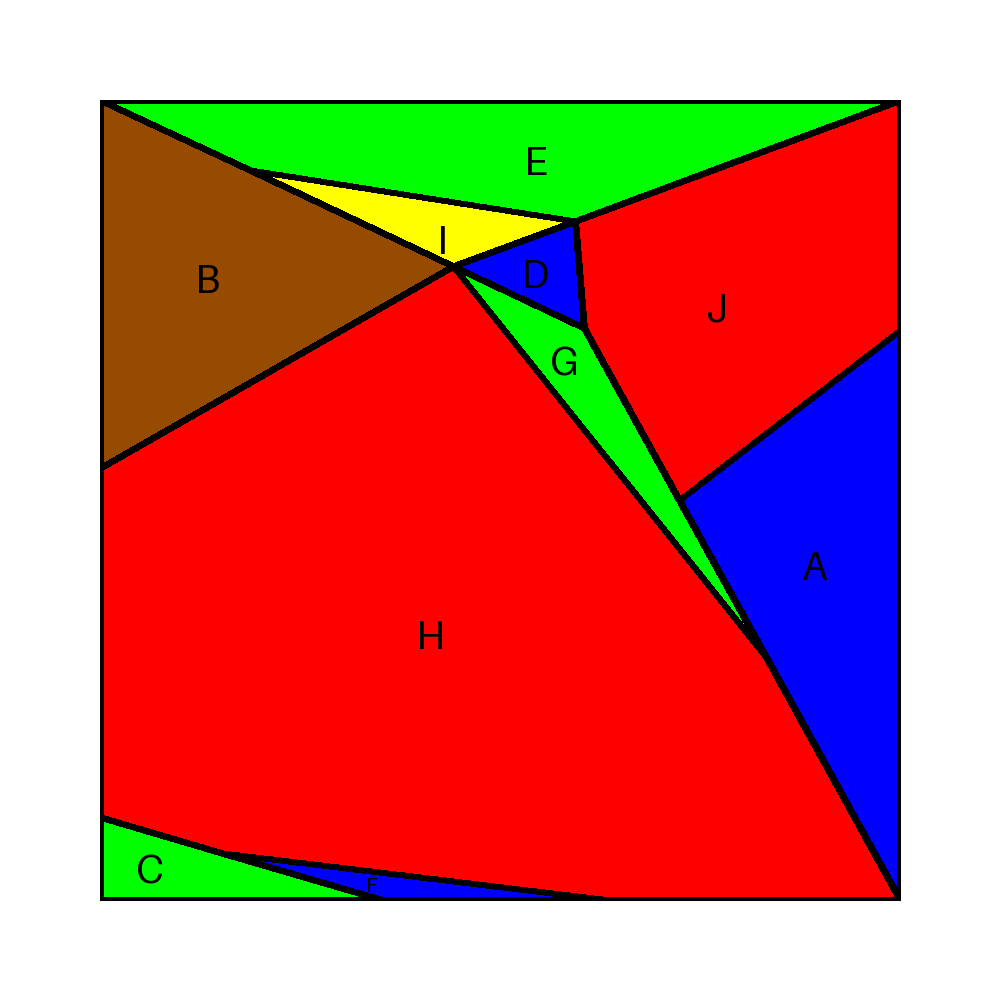
\includegraphics[height=4in]{Maps/RandomSetup1.png}
\end{center}

{\small  The diagram was created with the function 
call  {\tt TestQuestions.randomSetup(1)}.}

{\small The questions here and in the remaining examples were generated
by a call to function 
{\tt RandomQuestions.randomQuestions(5,$<${\it ExampleNumber}$>$)}.  The
first argument is the number of questions to be generated; the second is the
random seed.}

{\bf Question  22:} Let p be the meeting point of regions E, I, D, and J. Let q be the rightmost vertex of G. Let u be the rightmost vertex of F. Let v be the vertex at the bottom left of the overall diagram. Does the line segment between p and q cross the line segment between u and v? \\
{\bf Answer:}  No

{\bf Question  1:} Which regions border region B along an edge? \\
{\bf Answer:}  {I, E, H}

{\bf Question  23:} List all pairs of regions <X.Y> such that the bottom vertex of X is the same as the top vertex of Y. \\
{\bf Answer:}  [(I, G), (I, H), (E, D)]

{\bf Question  7:} Which regions, if any, meet the outside of the frame along two or more disconnected edges? \\
{\bf Answer:}  {H}

{\bf Question  15:} Let U be the union of regions B and E. Which of the labelled regions A-J does U border on an edge? \\
{\bf Answer:}  {I, J, H}

\pagebreak

\subsection{Example 3}
\begin{center}
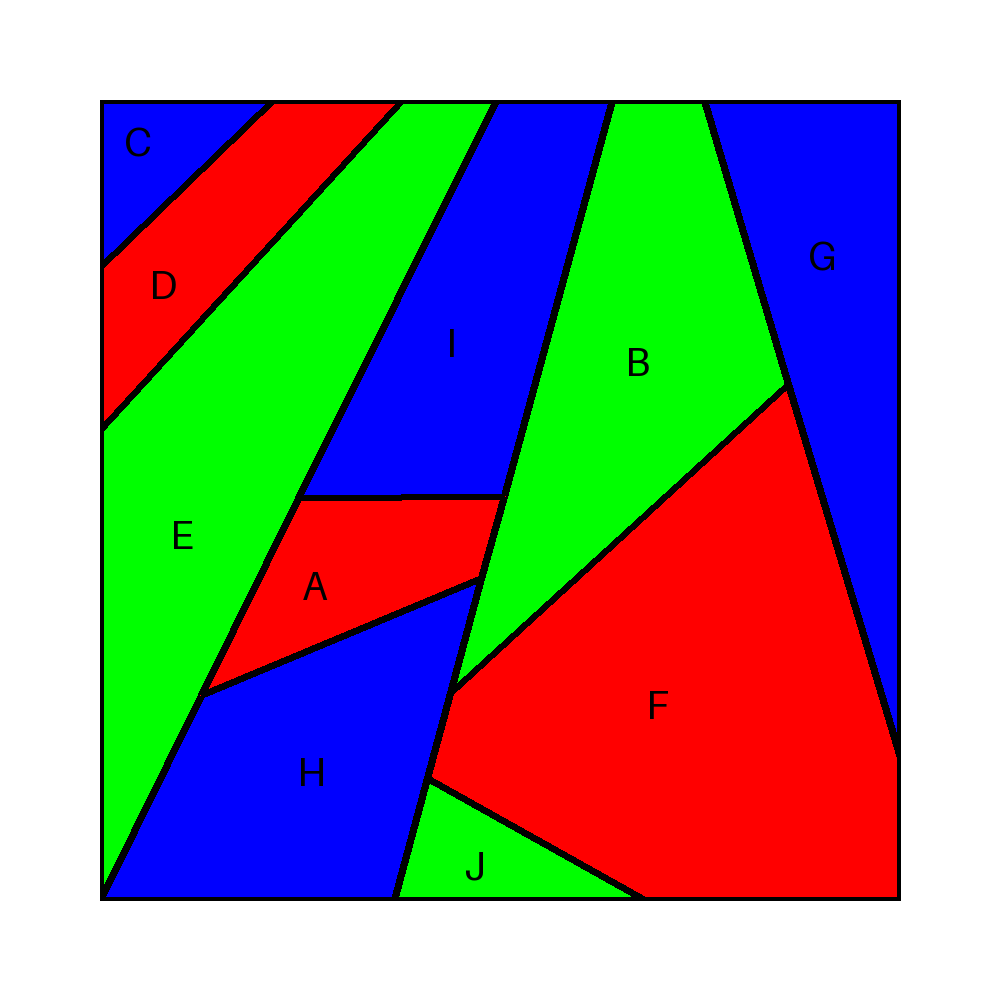
\includegraphics[height=4in]{Maps/RandomSetup2.png}
\end{center}

{\small  The diagram was created with the function 
call  {\tt TestQuestions.randomSetup(2)}.}


{\bf Question  23:} List all pairs of regions $<$X.Y$>$ such that the bottom vertex of X is the same as the top vertex of Y. \\
{\bf Answer:}  None

{\bf Question  13:} Let p be the leftmost vertex of I. Which regions meet at p? \\
{\bf Answer:}  ['I', 'E', 'A']

{\bf Question  18:} Let p be the vertex of G with the widest angle. Let q be the topmost vertex of H. If you travel in a straight line from p to q, what regions do you pass through in the interior, in sequence? (If you enter and exit a region more than once, list it multiple times.) \\
{\bf Answer:}  [G, B]

{\bf Question  16:} Sort regions [I, F, C, D] in order of increasing area: \\
{\bf Answer:}  [C, D, I, F]

{\bf Question  15:} Let U be the union of regions B and H. Which of the labelled regions A-J does U border on an edge? \\
{\bf Answer:}  {I, G, A, E, F, J}

\pagebreak

\subsection{Example 4}
\begin{center}
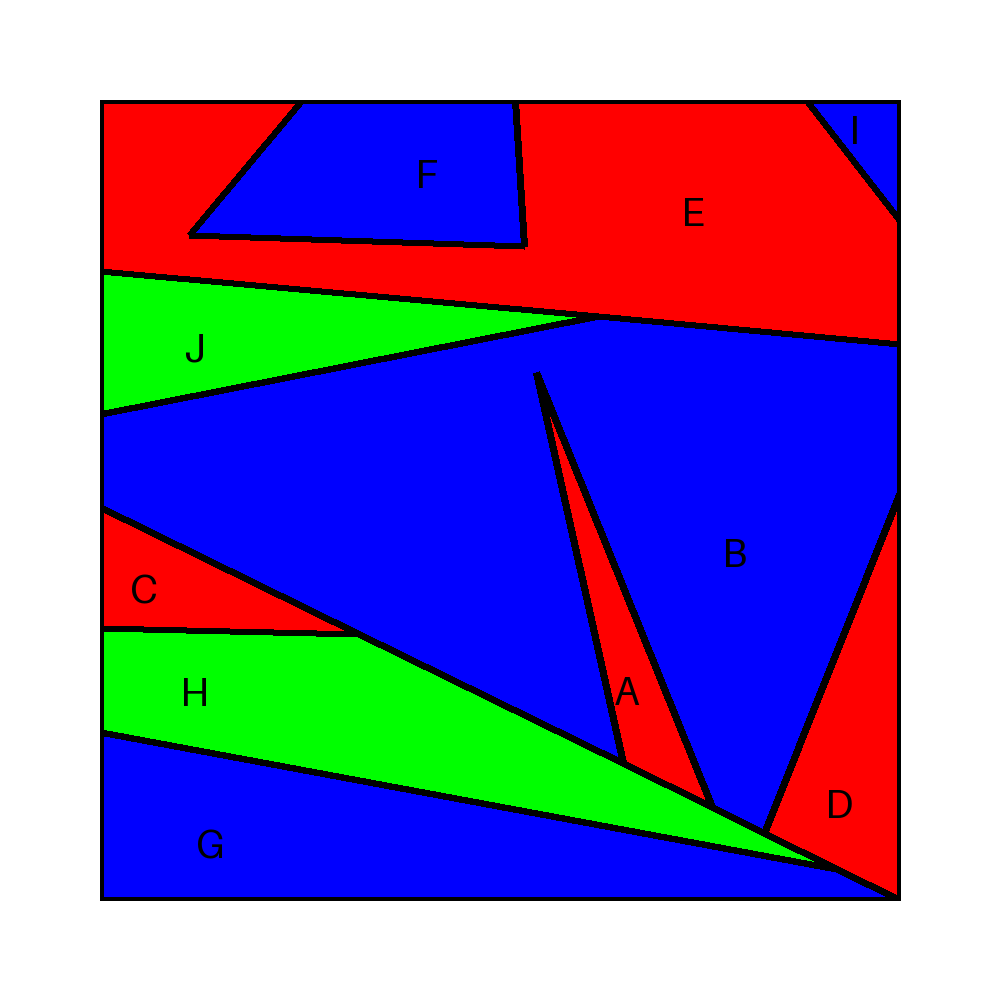
\includegraphics[height=4in]{Maps/RandomSetup3.png}
\end{center}

{\small  The diagram was created with the function 
call {\tt TestQuestions.randomSetup(3)}.}


{\bf Question  23:} List all pairs of regions <X.Y> such that the bottom vertex of X is the same as the top vertex of Y. \\
{\bf Answer:}  None

{\bf Question  22:} Let p be the vertex of F with the widest angle. Let q be the vertex at the bottom left of the overall diagram. Let u be the vertex of D with the widest angle. Let v be the top left vertex of J. Does the line segment between p and q cross the line segment between u and v? \\
{\bf Answer:}  Yes

{\bf Question  1:} Which regions border region I along an edge? \\
{\bf Answer:}  {E}

{\bf Question  4:} Let p be the vertex at the top left of the overall diagram. Suppose that someone starts at p and goes clockwise around E until they have returned to p. What regions do they pass on their left in sequence? For this question, include the outside of the frame. \\
{\bf Answer:}  [Outside, F, Outside, I, Outside, B, J, Outside]

{\bf Question  13}: Let p be the bottom right vertex of F. Which regions meet at p? \\
{\bf Answer:} ['F', 'E']


\pagebreak

\subsection{Example 5}
\begin{center}
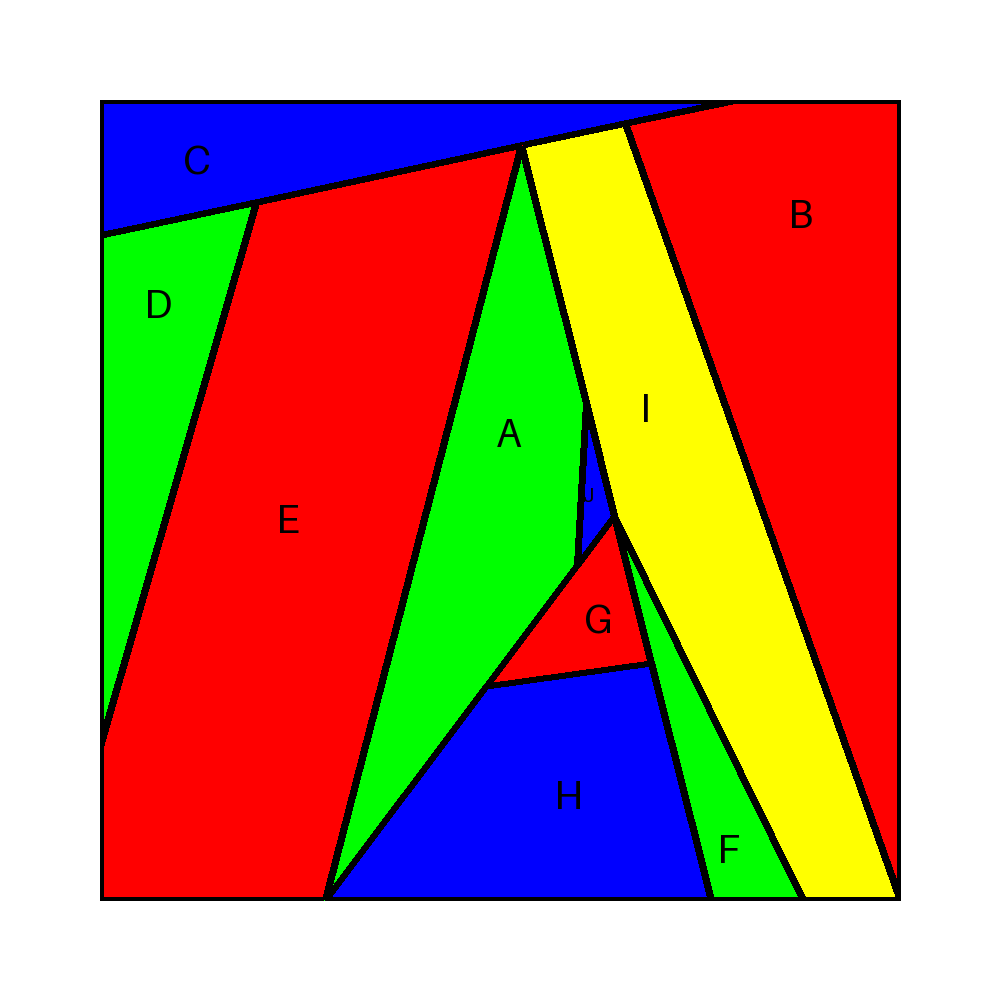
\includegraphics[height=4in]{Maps/RandomSetup4.png}
\end{center}

{\small  The diagram was created with the function 
call {\tt TestQuestions.randomSetup(4)}.}

{\bf Question  21:} Let u be the bottom left vertex of E. Let v be the vertex at the top right of the overall diagram. Let w be the vertex of D with the widest angle. Suppose that someone travels from u to v to w back to u.Is this cycle clockwise or counterclockwise? \\
{\bf Answer:}  counterclockwise

{\bf Question  3:} Which if any of the regions are not convex? \\
{\bf Answer:}  None

{\bf Question  19:} Let p be the bottommost vertex of D. Suppose that you travel in a horizontal line to the right from p until you reach the right side of the frame. What regions do you pass through in the interior, in sequence? (If you enter and exit a region more than once, list it multiple times.) \\
{\bf Answer:}  [E, A, H, F, I, B]

{\bf Question  20:} Let u be the bottom left vertex of E. Let v be the rightmost vertex of F. Let w be the vertex of H with the sharpest angle. Order u, v, and w in order left to right. \\
{\bf Answer:}  [u, w, v]

{\bf Question  24:} Which region is closer to B: G or D? (Consider the distance between two regions to be the distance between their closest points.) \\
{\bf Answer:}  G

\pagebreak

\subsection{Example 6}
\begin{center}
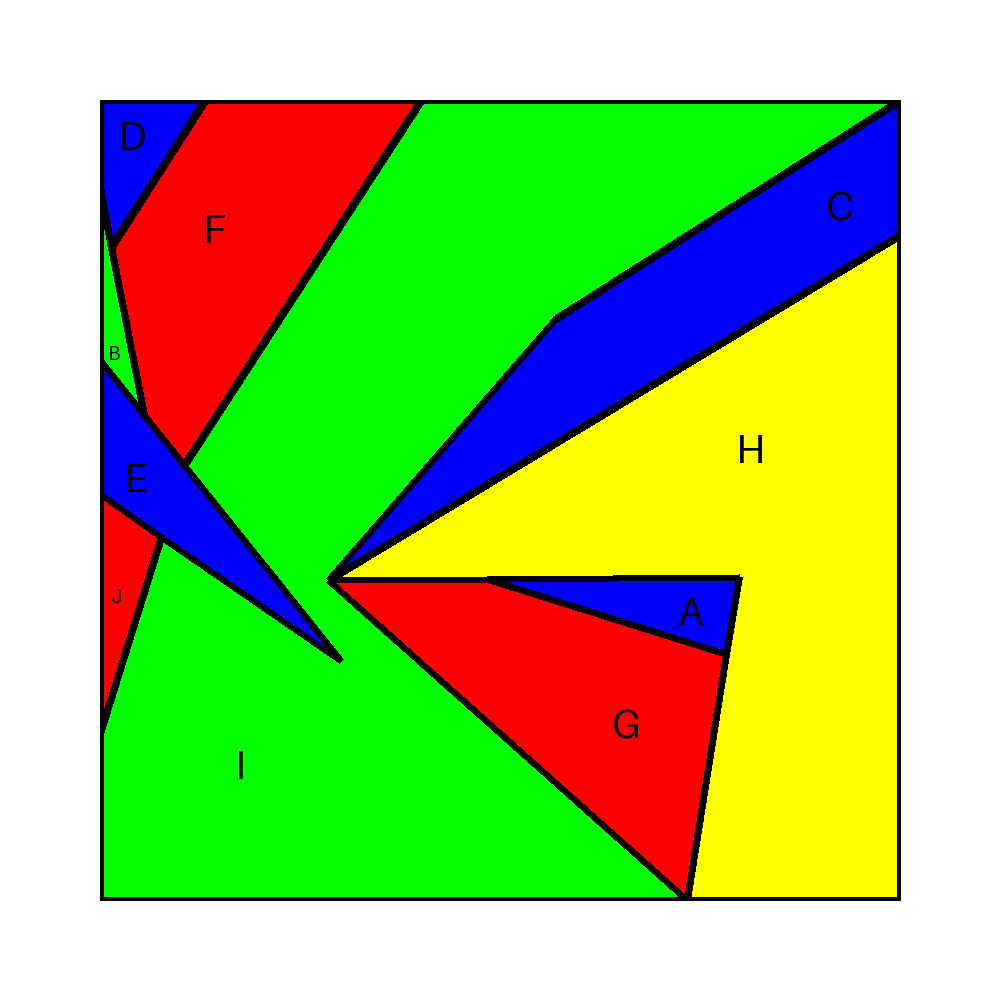
\includegraphics[height=4in]{Maps/RandomSetup5.png}
\end{center}

{\small  The diagram was created with the function 
call {\tt TestQuestions.randomSetup(5)}.}




{\bf Question  22:} Let p be the leftmost vertex of A. Let q be the bottommost vertex of E. Let u be the meeting point of regions F, E, and I. Let v be the topmost vertex of C. Does the line segment between p and q cross the line segment between u and v? \\
{\bf Answer:}  No 

{\bf Question  8:} Which regions have 4 sides? \\
{\bf Answer:}  {C, G, D} 

{\bf Question  6:} Which pairs of regions, if any, meet along two or more disconnected edges? Do not include the outside of the frame. \\
{\bf Answer:}  {(H, G)} 

{\bf Question  7:} Which regions, if any, meet the outside of the frame along two or more disconnected edges? \\
{\bf Answer:}  {I} 

{\bf Question  9:} How many sides does region B have? \\
{\bf Answer:}  3

\pagebreak

\subsection{Example 7}
\begin{center}
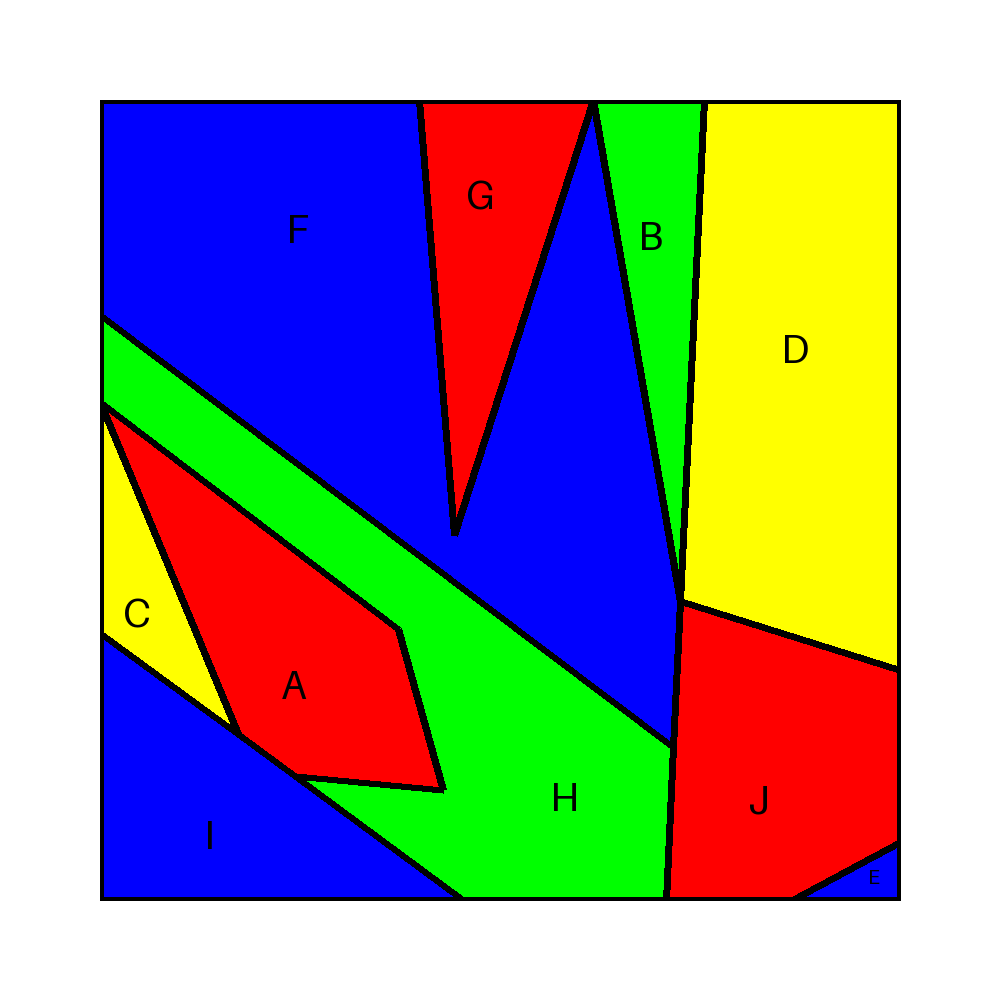
\includegraphics[height=4in]{Maps/RandomSetup6.png}
\end{center}

{\small  The diagram was created with the function 
call {\tt TestQuestions.randomSetup(6)}.}

{\bf Question  2:} If you draw a straight line segment from a point in the interior of region A to  a point in the interior of I, which other regions might it go through? \\
{\bf Answer:}  {H, C}

{\bf Question  12:} Let m be the edge of I that meets regions H, A, and C. Suppose m is extended in both directions along straight line L. Which are the regions R in the diagram for which L passes through the interior of R? (Do not include a region R if L only aligns with the boundary of R, and does not go through R's interior) \\
{\bf Answer:}  None

{\bf Question  14:} Let U be the union of regions A and H. How many sides does U have? \\
{\bf Answer:} 6

{\bf Question  3:} Which if any of the regions are not convex? \\
{\bf Answer:}  {H, F}

{\bf Question  22:} Let p be the meeting point of regions F, H, and J. Let q be the rightmost vertex of C. Let u be the top left vertex of G. Let v be the meeting point of regions B and D with the outside of the frame. Does the line segment between p and q cross the line segment between u and v? \\
{\bf Answer:}  No

\pagebreak

\subsection{Example 8}
\begin{center}
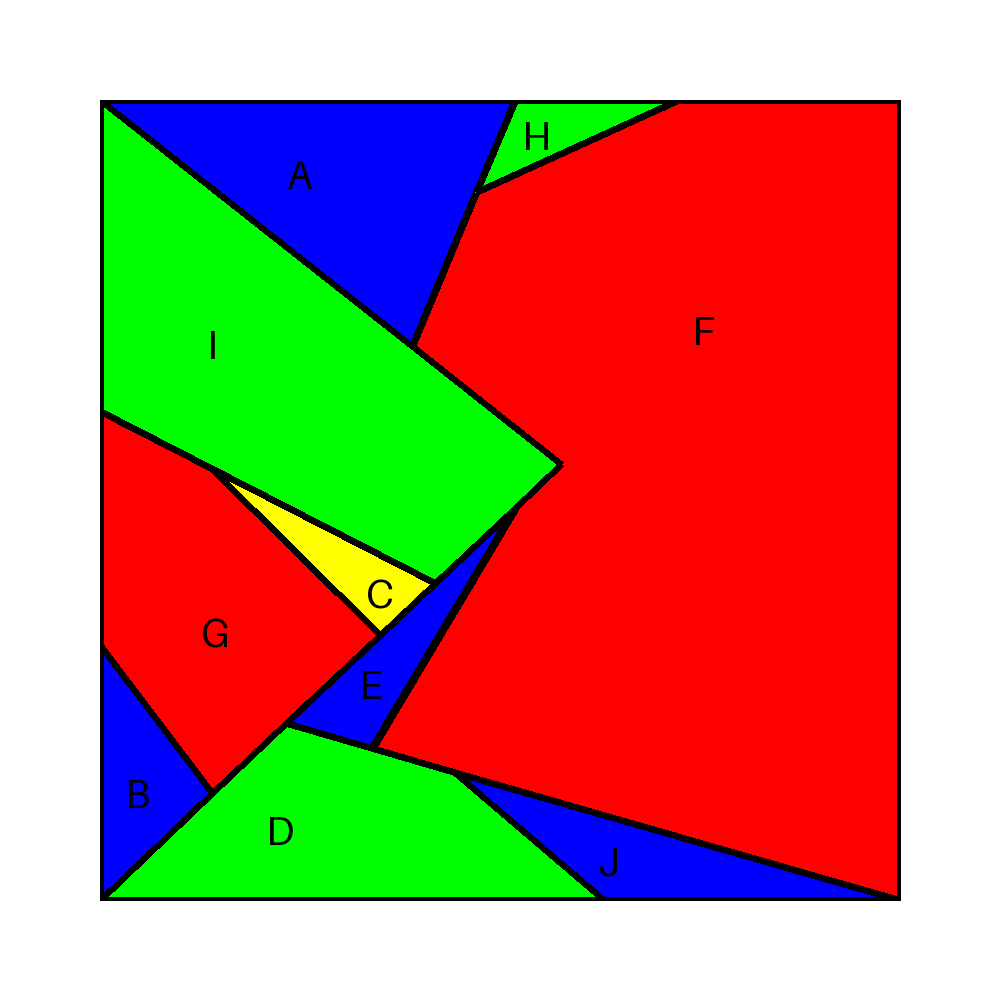
\includegraphics[height=4in]{Maps/RandomSetup7.png}
\end{center}

{\small  The diagram was created with the function 
call {\tt TestQuestions.randomSetup(7)}.}

{\bf Question  2:} If you draw a straight line segment from a point in the interior of region C to  a point in the interior of J, which other regions might it go through? \\
{\bf Answer:}  {G, E, F}

{\bf Question  12:} Let m be the rightmost edge of F. Suppose m is extended in both directions along straight line L. Which are the regions R in the diagram for which L passes through the interior of R? (Do not include a region R if L only aligns with the boundary of R, and does not go through R's interior) \\
{\bf Answer:}  None

{\bf Question  14:} Let U be the union of regions I and E. How many sides does U have? \\
{\bf Answer:}  7

{\bf Question  3:} Which if any of the regions are not convex? \\
{\bf Answer:}  {F}

{\bf Question  22:} Let p be the meeting point of regions H and F with the outside of the frame. Let q be the bottommost vertex of I. Let u be the meeting point of regions B and G with the outside of the frame. Let v be the topmost vertex of J. Does the line segment between p and q cross the line segment between u and v? \\
{\bf Answer:}  No

\pagebreak

\subsection{Example 9}
\begin{center}
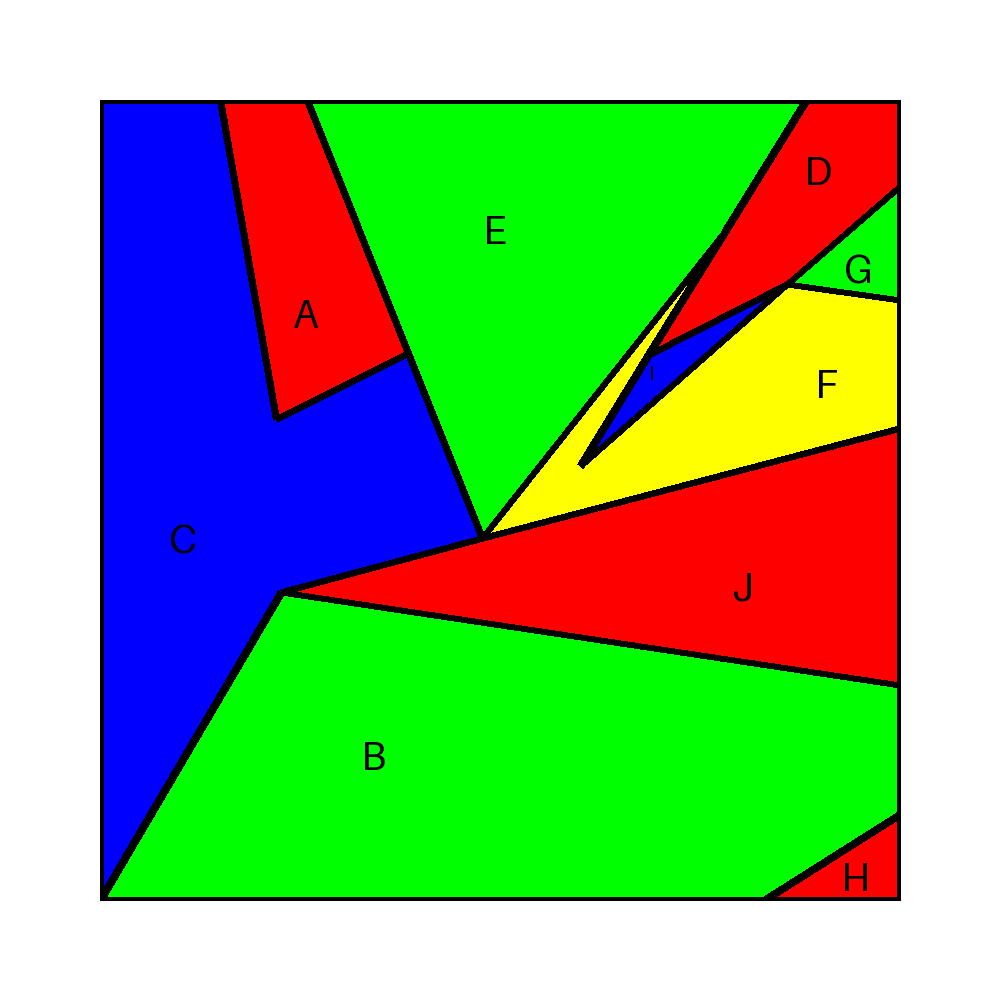
\includegraphics[height=4in]{Maps/RandomSetup8.png}
\end{center}

{\small  The diagram was created with the function 
call {\tt TestQuestions.randomSetup(8)}.}


{\bf Question  7:} Which regions, if any, meet the outside of the frame along two or more disconnected edges? \\
{\bf Answer:}  {B}

{\bf Question  8:} Which regions have 3 sides? \\
{\bf Answer:}  {G, J, I, H}

{\bf Question  5:} Which pairs of regions, if any, meet at a vertex but not along an edge? \\
{\bf Answer:}  {(F, C), (E, J), (I, G)}

{\bf Question  16:} Sort regions [A, J, C] in order of increasing area: \\
{\bf Answer:}  [A, J, C]

{\bf Question  1:} Which regions border region B along an edge? \\
{\bf Answer:}  {J, H, C}


\pagebreak

\subsection{Example 10}
\begin{center}
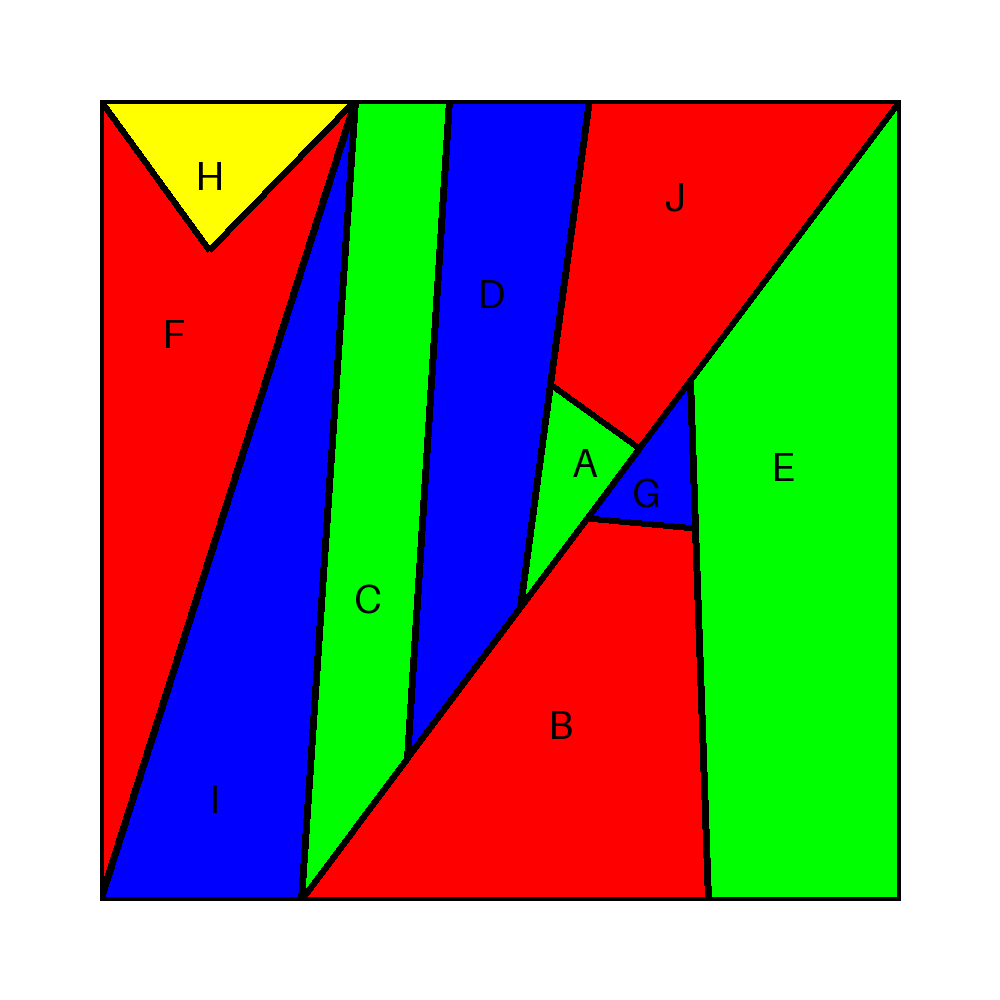
\includegraphics[height=4in]{Maps/RandomSetup10.png}
\end{center}

{\small  The diagram was created with the function 
call {\tt TestQuestions.randomSetup(10)}.}

{\bf Question  2:} If you draw a straight line segment from a point in the interior of region I to  a point in the interior of J, which other regions might it go through? \\
{\bf Answer:}  {D, A, C}

{\bf Question  8:}  Which regions have 4 sides? \\
{\bf Answer:}  {E, D, F, J, B, C}

{\bf Question  3:} Which if any of the regions are not convex? \\
{\bf Answer:}  {F}

{\bf Question  12:} Let m be the edge of D that meets regions A and J. Suppose m is extended in both directions along straight line L. Which are the regions R in the diagram for which L passes through the interior of R? (Do not include a region R if L only aligns with the boundary of R, and does not go through R's interior) \\
{\bf Answer:}  ['B']

{\bf Question  13:} Let p be the vertex of B with the widest angle. Which regions meet at p? \\
{\bf Answer:}  ['A', 'B', 'G']



\section{The Dataset}
\label{secBenchmark}
Code has been written to generate a dataset with a randomly constructed diagrams
and, for each diagram, randomly constructed questions from 24 different 
general templates together with their correct answers, as illustrated in

Given the range of possibilities, my guess would be that, if one were to
generate 800 random diagrams each with 10 regions, there would be few pairs 
if any that were not significantly different qualitatively. As a point of 
comparison, note that there are over a million planar graphs with 10 vertices,
so by the birthday paradox, one would need a set of a thousand randomly 
generated to have two that are identical. (This argument should not be taken
seriously for a number of reasons in opposite directions. On the one hand,
two maps that differ only in one bordering relationship are not very different;
and, though the procedure for generating random maps can generate any planar 
graph, there is certainly no reason to expect that it generates them 
equiprobably. On the other hand, two diagrams may have the same underlying 
connection graph and look very different qualitatively, and give very different
answers to the questions.)

\subsection{The Diagrams}
\label{secDiagrams}
Every diagram consists in a partition of an overall rectangle into irregular
polyhedral tiles. In the examples in section~\ref{secExamples}, the rectangles
are all squares and every diagram contains exactly 10 regions. However both the
aspect ratio of the rectangles and the number of regions is a parameter of a 
function call. 

Every region in the diagram is topologically homeomorphic to the unit disk; 
in other words, the boundary of every region is a topologically closed curve.
Any number of regions may meet at a vertex. Two regions may meet along a 
consecutive series of edges (for example, regions A and B in example 4)
or along multiple 
disconnected edges (for example, regions C and I in Example 1.) Most regions are
convex and have between 3 and 5 sides, but there are some non-convex regions 
(apparently about 1 in 10, with the current parameter settings) and some
regions with more than 5 sides. Regions are brightly colored blue, red, green,
yellow, brown, and possibly gray.\footnote{Of course, by the four-color theorem, tthe first four of these should suffice. The algorithm I have implemented 
certainly requires no more than six colors, and may in fact require no more
than five.} The 
coloring observes the constraints that no two regions that border on an
edge have the same color, and when easily achieved, that no two regions
that share a vertex have the same color. (In the examples in 
section~\ref{secExamples}, the second condition is always achieved.)
The regions are labelled with letters starting with 'A' in random order.

The intent of the benchmark is to create an overall map that humans can easily
read with questions that they can easily answer. Therefore the code is written
to avoid placing two vertices very close together, and to avoid generating 
angles very close to $0^{\circ}$ or to $180^{\circ}$. Nonetheless, with the
current parameters, we do end up with some very narrow regions that require 
letter labels in a smaller size that can be somewhat hard to see (e.g. region J
in example 5). 

The map is generated by iteratively choosing a region $R$ at random, with 
probability proportional to area($R$), and then 
splitting it into two parts using one of the splitting methods shown in 
figure~\ref{figSplits}. Table~\ref{tabBuildMap} shows the pseudo-code.

\begin{figure}
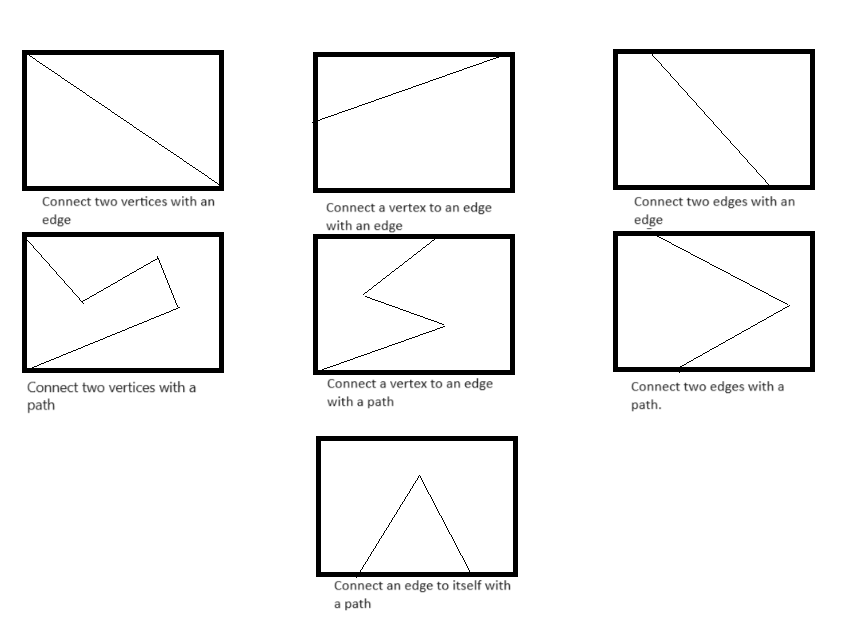
\includegraphics[height=4in]{FigSplits.png}
\caption{Ways to split a region}
\label{figSplits}
\end{figure}

\begin{table}
\begin{tabbing}
/* nRegions is the number of regions in the output map. \\
xSpan, ySpan are the dimensions of the overall rectanble */ \\
{\bf fun}\={\bf ction} BuildMap(nRegions,xSpan,ySpan) \{ \\
\> diagram $\leftarrow$ \{ rectangle(xSpan,ySpan) \} \\
\> {\bf for} \=i = 1:nRegions-1 \{ \\
\> \> f $\leftarrow$ randomly \=choose a region $R$ in diagram, \\
	\> \> \> with probability proportional to area($R$)  \\
\> \> randomly apply a splitting method to f generating new faces f1,f2 \\
\> \> diagram $\leftarrow$ diagram $\cup$ \{ f1,f2 \} $\setminus$ \{ f \} \\
\> \> \} \\
\> {\bf return} diagram \\
\}  
\end{tabbing}
\caption{Pseudo-code for constructing diagram}
\label{tabBuildMap}
\end{table}

Once the face has been selected, the random choice of a splitting method
involves (a) choosing the method type, following a fixed, non-uniform
distribution; (b) choosing the parameters of the method (the vertices/edges
involved; the positions along the chosen edges; and the number and locations of
intermediate points along the path).

Let $e(f)$ be the number of edges of region $f$. Suppose that you split
region $f$ into $f1$ and $f2$. If you use an edge-splitting method, then
you are guaranteed that $e(f1) \leq e(f)+1$, that $e(f2) \leq e(f)$,
that $e(f1)+e(f2) \leq e(f)+4$, and that, if $f$ is convex, then
both $f1$ and $f2$ are convex. However, if you used a path-splitting
method with $k$ intermediate vertices on the path, then 
$e(f)+2k+2 \leq e(f1)+e(f2) \leq e(f)+4$ and at least one of $f1$ or $f2$
must be non-convex. Therefore, one can indirectly control the number of
many-sided non-convex shapes that you generate by adjusting the probabilities
of the various methods. The examples shown above were generated using
a probability distribution over the seven method types shown in 
figure~\ref{figSplits} of [0.06,0.11,0.62,0.06,0.05,0.05,0.05]; thus,
there is a total probability of 0.21 of using a path-splitting method.
(We keep the probability of connecting vertex-to-vertex by an edge small
since these tend to oversimplify the diagram.) If you use a uniform distribution
over all splitting methods, you end up with diagrams like those in
figure~\ref{figComplex}; these may well be more complicated and harder to read
than you would want.

\begin{figure}
\includegraphics[width=6in]{Maps/Complex.png}
\caption{Complex diagram. Generated using uniform probabilities across the
seven methods with random seeds 1, 2, and 3}
\label{figComplex}
\end{figure}

(For replicability, the major functions here all include an argument to
set a random seed. It should be noted that, since many calls to the random
number generator are needed in the course of generating a diagram, apparently
small changes to the code may result in complete loss of replicability, as, 
of course, would changes to the RNG in the Python numpy library.)


\subsection{The Questions}
\label{secQuestions}
I have implemented code that, given a diagram, can generate questions following
24 different templates. Examples of all 24 current (8/17/24) templates
are given as part of Example 1,
above. I give an overview below of the question template set as currently
implemented, but of course all this is fairly easily modified 
with changes to the programming, so none of it is at all set in stone.

In the questions, regions are always identified by letter. Some questions
ask, or optionally ask, about pairwise unions of regions; these are always unions
of regions that meet along a consecutive sequence of edges, so that the
union is topologically a disk. E.g. in Example 1, there could be a question
about the union of C and G or the union of E and H, but not about the union
of B and H, which are disconnected, or about the union of C and I, which meet on
two disconnected edges, and whose union is therefore not simply connected.


Vertices are 
identified, either as the meeting place of regions, 
an extreme vertex of a region in some direction,  
or an extreme vertex of a region in terms of angle size. 
For instance Question 21 of Example 1 begins, 
``Let u be the meeting point of regions E and C with the outside of the 
frame. Let v be the vertex of H with the widest angle. Let w be the top 
left vertex of E.'' Some vertices cannot be named by any of these means; e.g.
in example 7, the common vertex of A and H that is closest to G is not
unique as a meeting point of A and H, nor is it extreme among the vertuces of
A or H in terms of angle or of any of the cardinal directions. Therefore, as
the code is currently written, no question about this vertex can be formulated.
(Of course it would be possible to extend the code to allow expressions like
``the common vertex of A and H that is closest to G''; the question is, what
kinds of such extensions would you want to permit?) When a vertex can be named
in multiple ways --- e.g. in the example above, vertex w could just as well
have been identified as ``the meeting point of H, I, and C'', `the bottom
vertex of H'' or ``the rightmost vertex of C'' --- the choice is made
at random.

A number of questions refer to lines or line segments. These can be identified
either as the line segment between two specified vertices; as
the ray starting at a specified vertex and moving in a specified cardinal
direction; as all lines between the interior of two specified regions; or
as the continuation of an edge, which in turn may be
specified either as the boundary between two region or as the extreme border
of a region in some cardinal direction.

The form of the answer may be
(a) Boolean or binary choice 
(b) a small integer; 
(c) a region; 
(d) a set of regions; 
(e) an ordered list of regions; 
(f) an ordered list of vertices; 
(g) a set of pairs of faces. 

The geometric features that the questions refer to, or ask about, include
topological features; number of sides; comparative distances; comparative
angle; comparative position in a cardinal direction;
comparative area; clockwise vs. counterclockwise triples of points; 
convexity; and lines crossing the interior of regions or two lines 
crossing each other.

Table~\ref{tabQuestions} shows the features of each
question, other than those involved in vertex identification.

Some questions can only be asked in one form for each diagram, 
e.g. question 3, ``Which
if any of the regions are not convex?''. Most have multiple instances per
diagram; e.g. Question 1, ``Which regions border region $<$ identifier $>$ 
on an edge?''

\begin{table}
\begin{center}
\begin{tabular}{|l|l|l|l|l|} \hline
Q & Answer form     & Features & Unique? & Line identification \\ \hline
1 & Set of regions  & Topology & Yes     & \\ \hline
2 & Set of regions  & Line crossing & No & Lines between \\ 
  &                 &               &    & region interior \\ \hline
3 & Set of regions  & Convexity & Yes    &  \\ \hline
4 & List of regions & Topology  & No     &  \\ \hline
5 & Set of pairs of regions & Topology & Yes & \\ \hline
6 & Set of pairs of regions & Topology & Yes & \\ \hline
7 & Set of region   & Topology & Yes & \\ \hline
8 & Set of regions  & Number of sides & Yes & \\ \hline
9 & Small integer   & Number of sides & Yes & \\ \hline
10 & List of vertices & Distance & No & \\ \hline
11 & List of vertices & Angle size & No & \\ \hline
12 & List of vertices & Line crossing & No & Extension of edge\\ \hline
13 & Set of regions &  Topology & No & \\ \hline
14 & Small integer  & Number of sides & No & \\ \hline
   &                & Union of region &    & \\ \hline
15 & Set of regions & Topology        & No & \\ 
   &                & Union of regions & & \\ \hline
16 & List of regions & Area of regions & No & \\\hline
17 & Set of pairs of regions & Union of regions& No & \\ \hline
	&                         & Convexity & No & \\ \hline
18 & List of regions & Line crossing & No  & Endpoints \\
   &                 &               &     & specified \\ \hline
19 & List of regions & Line crossing & No & Endpoint and \\
   &                 &               &     & direction \\ \hline
20 & List of vertices & Position in  & No &            \\
   &                 & cardinal direction & & \\ \hline
21 & Binary choice  & Clockwise      & No & \\ \hline
22 & Boolean        & Line crossing  & No   & Endpoint \\
   &                 &               &     & specified \\ \hline
23 & List of pairs of regions & Position in    & Yes & \\ \hline
24 & Binary choice   & Distance & No & \\ \hline
\end{tabular}
\end{center}
\caption{Features of question templates. The features used in
in identifying vertices are not included nere. The ``Unique?'' column
is ``Yes'' if there is only one instance of this question per
diagram} 
\label{tabQuestions}
\end{table}

I have made a substantial effort, in writing the code, to ensure that
the questions are easily answerable by humans (just using my own subjective
judgment). I think I have been largely successful but certainly not entirely.
An extreme example --- so extreme that it really qualifies as a bug ---
is question 2 in example 8. It is really not obvious under visual inspection
that a line from just inside the upper left corner of J to just inside the
the upper left corner of C passes through the interior of G, though it is easily
verified using drawing software. 

\subsection{The Code, so far}
\label{secCode}
The code is in Python --- currently about 4000 lines. It seems to be largely 
debugged, but I have no reason to suppose, and would be very surprised to learn,
that it is completely debugged. It is almost completely uncommented, except
for noting a few fiddly points that I myself might quickly forget. This is the
first substantial program I've written in Python, so no doubt there are
plenty of unnecessary inefficiencies and stylistic uglinesses. There is at
least one deprecated and outdated method, namely the use of {\tt numpy.random}.




\section{Where should we take this?}
\label{secFuture}

Broadly speaking, I would like to use this as a benchmark for VQA AI systems. 
This will certainly be done much better and more usefully if I can work with
collaborators who are more knowledgeable and more experienced than me (that 
bar is pretty much on the floor.)

\pagebreak

Decisions to be made include:
\begin{itemize}
\item How should the answers be formulated: Free form, explicitly specified
form, multiple choice, binary choice? With questions whose answer is a
set or a list, is partial credit given and if so, how?

\item How is the dataset to be divided into a training set and a test set?
Options include: 
\begin{itemize}
\item[(a)] Use this only as a test set, not as a training set.
\item[(b)] Choose randomly among diagram-question pairs. Thus, the training set will
contain every diagram type and every question type, but not every combination.
\item[(c)] Include all questions types but only some of the diagrams 
in the training set, thus forcing the AI to generalize to new diagrams.
\item[(d)] Include all of the diagrams but only some of the question types,
thus forcing the AI to generalize to new question types.
\item[(e)] Include only some of the diagrams and some of the question types,
forcing the AI to generalize in both directions.
\end{itemize}

\item What should be tested? Models, training, fine-tuning, prompts, etc.

\item Should we do human subject tests? If so, how? In particular, should we
do tests of human subjects who can use drawing software to draw straight lines?

\item Where should we set the bar in trying to make the problems easy for
humans, and how?
\end{itemize}
\end{document}



